\documentclass[11pt]{article}
\usepackage[T1]{fontenc}
\usepackage{newtxtext}
\usepackage[margin=1in,headheight=15pt]{geometry}
\usepackage{microtype}
\usepackage{amsmath,amsthm,mathtools}
\usepackage{newtxmath}
\usepackage{graphicx,booktabs,array,longtable}
\usepackage{xcolor}
\usepackage{enumitem}
\usepackage{fancyhdr}
\usepackage{hyperref}
\usepackage{bookmark}
\usepackage{titlesec,needspace}
\definecolor{ink}{HTML}{17324D}
\definecolor{muted}{HTML}{566573}
\hypersetup{colorlinks=true,linkcolor=ink,citecolor=ink,urlcolor=ink,
 pdftitle={First Pattern Failure in Catalan Permutations},
 pdfauthor={Research report prepared for Vladimir Reshetnikov},
 pdfsubject={A proof of OEIS A273821, exact enumeration, asymptotics and a critical phase transition}}
\titleformat{\section}{\large\sffamily\bfseries\color{ink}}{\thesection}{0.7em}{}
\titleformat{\subsection}{\normalsize\sffamily\bfseries\color{ink}}{\thesubsection}{0.7em}{}
\pagestyle{fancy}
\fancyhf{}
\fancyhead[L]{\small\sffamily A273821: exact enumeration and critical behavior}
\fancyhead[R]{\small\sffamily Research report}
\fancyfoot[C]{\small\thepage}
\renewcommand{\headrulewidth}{0.3pt}
\setlength{\parskip}{4pt}
\setlength{\parindent}{1em}
\setlength{\emergencystretch}{2em}
\setcounter{tocdepth}{2}
\numberwithin{equation}{section}
\newtheorem{theorem}{Theorem}[section]
\newtheorem{lemma}[theorem]{Lemma}
\newtheorem{proposition}[theorem]{Proposition}
\newtheorem{corollary}[theorem]{Corollary}
\theoremstyle{definition}
\newtheorem{definition}[theorem]{Definition}
\newtheorem{remark}[theorem]{Remark}
\newcommand{\Av}{\operatorname{Av}}
\newcommand{\E}{\mathbb E}
\newcommand{\Prob}{\mathbb P}
\newcommand{\fall}[2]{(#1)_{\underline{#2}}}
\newcommand{\coeff}[2]{[#1^{#2}]}
\newcommand{\dd}{\mathrm d}
\newcommand{\Beta}{\operatorname{Beta}}
\newcommand{\Li}{\mathcal L}
\newcommand{\ind}{\mathbf 1}
\newcommand{\Cat}{\mathcal C}
\newcommand{\Oeis}[1]{\href{https://oeis.org/#1}{\texttt{#1}}}
\newcommand{\smallurl}[1]{{\small\url{#1}}}

\begin{document}
\begin{titlepage}
\vspace*{0.6in}
{\sffamily\small\bfseries\color{muted} OEIS RESEARCH \quad / \quad EXACT ENUMERATION AND ASYMPTOTICS\par}
\vspace{0.45in}
{\sffamily\bfseries\color{ink}\fontsize{27}{33}\selectfont
First Pattern Failure\par
in Catalan Permutations\par}
\vspace{0.25in}
{\Large A proof of OEIS A273821, exact formulas,\par
all-orders expansions, and a critical phase transition\par}
\vspace{0.4in}
{\large Research report prepared for Vladimir Reshetnikov\par}
{\normalsize October 1, 2026\par}
\vspace{0.5in}
\hrule
\vspace{0.2in}
\begin{abstract}
For a uniformly chosen $123$-avoiding permutation of $[n]$, let $K_n$ be the
largest number of its largest entries whose induced permutation still avoids
$132$. The generating function for the joint counts $T(n,k)$ is marked
conjectural in OEIS A273821. We prove it by inserting successive minima,
then telescope the resulting Catalan convolution to obtain a difference of
two binomial coefficients. This resolves both the posted generating-function
conjecture and the indicated growth-rate question for every nonzero fixed
column.

The exact formula yields substantially more: every column $k\ge2$ is
hypergeometric in $n$; its full inverse-power expansion is computable to any
order; and $K_n$ has an explicit discrete limit law with exponentially
weighted total-variation error $O(n^{-1})$. The fixed-column approximation
changes at $k\asymp\sqrt n$, where we prove an explicit crossover. For
$k$ proportional to $n$, two distinct exponential sectors are separated
exactly rather than hidden under an algebraic error term.

Weighting permutations by $y^{K_n}$ produces a transition at $y=2$.
Below the transition $K_n$ stays bounded; above it $n-K_n$ stays bounded;
at the transition $K_n/n$ converges to $\Beta(1,\tfrac12)$. We give an exact
critical partition function and mean, a critical window, Lambert-$W$
inverse expansions, independent computation, and a formalization and research
agenda.
\end{abstract}
\vfill
{\small\color{muted}
\textbf{Status.} The report supplies conventional proofs and executable checks,
not a Lean formalization. The identified OEIS conjecture is proved here;
priority for every extension is not certified by an exhaustive literature
search. No OEIS edit or repository change has been submitted.\par}
\end{titlepage}

\tableofcontents
\newpage

\section{The question, the answer, and the scope of the claim}

\subsection{The statistic and the live OEIS question}
A permutation avoids a pattern if no subsequence, with positions increasing,
has the same relative order as that pattern. Thus $123$ avoidance forbids
three increasing entries, and $132$ avoidance forbids indices $i<j<h$ with
$\pi_i<\pi_h<\pi_j$. Write $\Av_n(123)$ for the first class.

For $\pi\in\Av_n(123)$, restrict $\pi$ to its $k$ largest values without
changing their order. Let $K(\pi)$ be the largest $k$ for which this
restriction avoids $132$. Set
\begin{equation}\label{eq:definition}
 T(n,k)=\#\{\pi\in\Av_n(123):K(\pi)=k\},\qquad
 Z_n(y)=\sum_{k=1}^n T(n,k)y^k.
\end{equation}
The triangle is \Oeis{A273821}, introduced by David Callan in 2016
\cite{oeis273821}. As retrieved on October 1, 2026, its bivariate generating
function remains labeled conjectural; its comments also suggest growth
constant $4$ for each column other than the first. These are the two
specific posted questions answered below.

We use $C_n=\frac1{n+1}\binom{2n}{n}$ and
\begin{equation}\label{eq:catalan}
 C(x)=\sum_{n\ge0}C_nx^n=\frac{2}{1+\sqrt{1-4x}},
 \qquad C(x)=1+xC(x)^2.
\end{equation}
Our insertion argument will itself establish the Catalan row sums, so the
proof does not assume the conjectural triangle recurrence or generating
function. All entries outside $1\le k\le n$ are zero. For a binomial
coefficient with nonnegative upper argument, a negative lower argument is
interpreted as zero.

\subsection{Principal conclusions}
The central enumeration result is
\begin{equation}\label{eq:main-binomial}
\boxed{\displaystyle
 T(n,k)=2^{k-1}\binom{2n-2k}{n-k-1}
             -\binom{2n-k-1}{n-k-1}\quad (n>k\ge1),}
\end{equation}
with the separate diagonal value $T(n,n)=2^{n-1}$. In particular, the first
column is zero after its initial entry.

The resulting bivariate generating function is
\begin{equation}\label{eq:main-gf}
\boxed{\displaystyle
 F(x,y):=\sum_{n\ge1}Z_n(y)x^n
 =\frac{xy}{1-2xy}
  +\frac{x^3y^2C(x)^3}{(1-2xy)(1-xyC(x))}.}
\end{equation}
This is algebraically the conjectured OEIS expression. Its present form
records the first failure of $132$ avoidance explicitly.

For every fixed $k\ge2$,
\begin{equation}\label{eq:main-asymptotic}
 T(n,k)\sim \frac{(k-1)(k+4)}{2^{k+3}\sqrt\pi}\,
                 \frac{4^n}{n^{3/2}}.
\end{equation}
We prove a full expansion with explicit first coefficients and an all-orders
recursion, not only this leading equivalent. Moreover, for a uniform
permutation in $\Av_n(123)$,
\begin{equation}\label{eq:main-discrete-law}
 \Prob(K_n=k)\longrightarrow p_k:=\frac{(k-1)(k+4)}{2^{k+3}}
 \quad(k\ge2),\qquad
 \sum_{k\ge2}p_ky^k=\frac{y^2(3-y)}{2(2-y)^3}.
\end{equation}

There is a second, macroscopic phenomenon. Under the probability measure
proportional to $y^{K(\pi)}$, the scaling of $K_n$ changes at $y=2$:
\begin{equation}\label{eq:phase-summary}
\begin{array}{c|c}
 0<y<2 & K_n\text{ converges to an explicit discrete law},\\[2pt]
 y=2 & K_n/n\ \Rightarrow\ \Beta(1,\tfrac12),\\[2pt]
 y>2 & n-K_n\text{ converges to an explicit discrete law}.
\end{array}
\end{equation}
The critical normalization has the exact evaluation
\begin{equation}\label{eq:critical-preview}
 Z_n(2)=(n+2)\binom{2n}{n}-4^n.
\end{equation}
These conclusions are consequences of the same exact first-failure
formula, not independent guesses from numerical plots.

\subsection{What is established, and what is not claimed}
The contribution is a self-contained resolution of an identifiable posted
conjecture, together with a detailed analysis of its refined counting
triangle. Pattern-avoiding permutations, Catalan generating trees, Stirling
expansions, and singularity analysis are established methods; they are not
claimed as new here. The two low columns already have known companion
entries, \Oeis{A000245} and \Oeis{A071718}, including known leading
asymptotics \cite{oeis245,oeis71718}.

A targeted search of the sequence identifier and defining statistic did
not locate an independent published proof of the A273821 conjecture.
That is a limited search result, not a proof of priority. Accordingly,
``proved here'' is used literally, while an assertion that every extension
is unprecedented is deliberately avoided.

The ProveIt repository has an independent transseries library for asymptotic
scales and differential blocks, together with an inversion volume, a
combinatorial companion, and verification programs \cite{proveit}. Here we
distinguish formal expansions, analytic interpretation, and executable
checks, especially when an exponentially smaller sector is present. No theorem from the
repository is needed as an unverified premise, and none of the results
below is represented as already formalized in Lean.

\section{A minimum-insertion model for Catalan permutations}

\subsection{The active suffix}
Every nonempty permutation has a unique parent obtained by deleting its
minimum and standardizing the remaining values. Reversing this operation
builds a permutation by inserting successively smaller values.

\begin{definition}
The suffix state $d$ of a nonempty permutation is the length of its longest
terminal decreasing subsequence of \emph{consecutive positions}. Thus the
last $d$ entries decrease, and either the permutation is decreasing or the
entry immediately before them forms an ascent with the first of those $d$
entries. An insertion site is indexed by the number $j$ of old entries to
its right.
\end{definition}

\begin{lemma}[Active sites]\label{lem:active}
For a permutation in $\Av_n(123)$ with suffix state $d$, insertion of a new
minimum preserves $123$ avoidance exactly at the sites $0\le j\le d$.
The new state is $d+1$ when $j=0$, and is $j$ when $1\le j\le d$.
Consequently the state production rule is
\begin{equation}\label{eq:production}
 d\longrightarrow 1,2,\ldots,d,d+1,
\end{equation}
with each child state occurring once.
\end{lemma}
\begin{proof}
Any newly formed increasing triple must start at the new minimum. Such a
triple exists precisely when the entries to its right contain an increasing
pair. Avoiding such a pair means that this right-hand suffix is decreasing,
which is equivalent to $j\le d$. If the minimum is appended, it lengthens
the decreasing suffix by one. Otherwise it lies just before a decreasing
suffix of length $j$ and is smaller than its first entry, so that suffix
cannot extend to the left. Its new length is exactly $j$.
\end{proof}

\subsection{Descendant generating functions}
Let $D_d(x)$ count descendants of a state-$d$ permutation, with $x$ marking
the number of additional minima inserted. The particular values or earlier
shape of the permutation do not matter, because the production rule depends
only on $d$.

\begin{lemma}\label{lem:descendants}
For every $d\ge1$,
\begin{equation}\label{eq:descendants}
 D_d(x)=C(x)^{d+1}.
\end{equation}
\end{lemma}
\begin{proof}
The production rule gives
\[
 D_d(x)=1+x\sum_{j=1}^{d+1}D_j(x).
\]
This infinite system has a unique formal-power-series solution with constant
term $1$: after the coefficients through degree $m-1$ have been determined
for every state, the equation determines the coefficient of degree $m$
for every state using only a finite sum. To verify the claimed solution,
use $xC^2=C-1$:
\[
 x\sum_{j=1}^{d+1}C^{j+1}
 =(C-1)(1+C+\cdots+C^d)=C^{d+1}-1.
\]
Uniqueness finishes the proof.
\end{proof}
The single-entry permutation has state $1$. Therefore the number of
size-$n$ permutations generated is
\[
 [x^{n-1}]D_1(x)=[x^{n-1}]C(x)^2=C_n,
\]
where the final equality follows from $xC^2=C-1$. Thus this construction
also proves the Catalan row sums.

\subsection{The two safe sites for avoiding both patterns}
Suppose the current permutation avoids both $123$ and $132$. At an active
site the entries to the right of a newly inserted minimum decrease. The new
minimum starts a $132$ occurrence exactly when there are at least two such
entries. Hence the insertions that remain safe for both patterns are
precisely $j=0$ and $j=1$.

The first appends the new minimum and increases $d$ by one; the second places
it before the last entry and resets $d$ to $1$. These two choices encode
all size-$k$ safe prefixes by binary words of length $k-1$.

\begin{lemma}\label{lem:safe-count}
Let $a_{k,d}$ be the number of permutations of size $k$ avoiding both
patterns and having suffix state $d$. Then
\begin{equation}\label{eq:safe-count}
 a_{k,k}=1,\qquad a_{k,d}=2^{k-d-1}\quad(1\le d<k).
\end{equation}
In particular, there are $2^{k-1}$ such permutations, and for $2\le j\le k$,
\begin{equation}\label{eq:safe-tail}
 \sum_{d=j}^k a_{k,d}=2^{k-j}.
\end{equation}
\end{lemma}
\begin{proof}
The state is $k$ only if every insertion appends. Otherwise locate the last
reset: to finish at state $d<k$ it must be followed by exactly $d-1$
appends. The preceding $k-d-1$ decisions are free. Summation gives both
remaining assertions.
\end{proof}

\section{First failure and the conjectured generating function}

\subsection{The first-failure decomposition}
Once a $132$ occurrence has appeared among the largest entries, inserting
smaller entries cannot remove it. Thus $K=k<n$ is equivalent to remaining
safe through size $k$ and failing at the next insertion. At that failure
insertion the active site has $j\ge2$ entries to its right.

\begin{theorem}[Positive Catalan convolution]\label{thm:convolution}
For $n>k\ge2$,
\begin{equation}\label{eq:convolution}
 T(n,k)=\sum_{j=2}^k 2^{k-j}[x^{n-k-1}]C(x)^{j+1}.
\end{equation}
For $n=k$, $T(n,n)=2^{n-1}$; for $n>1$, $T(n,1)=0$.
\end{theorem}
\begin{proof}
For a fixed failing site $j$, a safe size-$k$ prefix permits that insertion
exactly when its state $d$ satisfies $d\ge j$. There are $2^{k-j}$ such
prefixes by Lemma~\ref{lem:safe-count}. The failing insertion gives state
$j$ by Lemma~\ref{lem:active}; the remaining $n-k-1$ insertions are arbitrary
$123$-preserving descendants and are counted by $C^{j+1}$. The parent
operation is unique, so these cases are disjoint and exhaustive. The
boundary cases follow from the safe-prefix count and the fact that a
$132$ occurrence needs three entries.
\end{proof}

For example, the row at size $5$ is
\[
(T(5,1),\ldots,T(5,5))=(0,9,10,7,16).
\]
The off-diagonal formula gives $T(5,3)=[x](2C^3+C^4)=6+4=10$.
The row sums to $42=C_5$. This example is computed from the insertion
argument, not used to infer it.

\subsection{Summation of the columns}
\begin{theorem}[Proof of the posted generating-function conjecture]
The identity \eqref{eq:main-gf} holds in $\mathbb Q[y][[x]]$. It is equal to
\begin{equation}\label{eq:oeis-gf}
 C(x)-1+
 \frac{(1-y)(1-xy)\{1-(1-xy)C(x)\}}
 {(1-2xy)(1-y+xy^2)},
\end{equation}
the expression marked conjectural in OEIS A273821 \cite{oeis273821}.
\end{theorem}
\begin{proof}
The size generating function for column $k$ is
\begin{equation}\label{eq:column-gf}
 G_k(x)=2^{k-1}x^k+x^{k+1}\sum_{j=2}^k2^{k-j}C(x)^{j+1},
 \qquad G_1(x)=x.
\end{equation}
The diagonal contribution sums to $xy/(1-2xy)$. In the second contribution,
write $k=j+h$ and sum the two geometric series:
\begin{align*}
 \sum_{k\ge2}y^kx^{k+1}\sum_{j=2}^k2^{k-j}C^{j+1}
 &=xC\sum_{j\ge2}(xyC)^j\sum_{h\ge0}(2xy)^h\\
 &=\frac{x^3y^2C^3}{(1-2xy)(1-xyC)}.
\end{align*}
This proves \eqref{eq:main-gf}. To compare with \eqref{eq:oeis-gf}, replace
$xC^2$ by $C-1$ and use
\[
 1-y+xy^2=(1-xyC)(1-y/C).
\]
Clearing denominators then gives identical numerators. This is an identity
of rational algebraic functions; any removable factors in the displayed
OEIS form are interpreted through the formal series \eqref{eq:main-gf}.
\end{proof}
Setting $y=1$ gives $F(x,1)=C(x)-1$, consistently with the combinatorial
row-sum proof. The derivation also shows why two apparently different
singular factors occur: $1-2xy$ records the binary safe-prefix evolution,
whereas $1-xyC$ records the active suffix at first failure.

\section{Two binomials, exact tails, and hypergeometric columns}

\subsection{A telescoping Catalan convolution}
Lagrange inversion applied to $C=1+xC^2$ gives, for $m\ge0$ and $j\ge1$,
\begin{equation}\label{eq:ballot}
 b(m,j):=[x^m]C(x)^{j+1}
 =\frac{j+1}{2m+j+1}\binom{2m+j+1}{m}
 =\binom{2m+j}{m}-\binom{2m+j}{m-1}.
\end{equation}
For completeness, if $m>0$, set $u=C-1=x(1+u)^2$. The Lagrange formula
for $[x^m](1+u)^{j+1}$ is
$\frac{j+1}{m}[u^{m-1}](1+u)^{2m+j}$, which simplifies to the first
expression. At $m=0$ both sides are $1$.

\begin{lemma}[Telescoper]\label{lem:telescoper}
For $t_j=2^{-j}\binom{2m+j}{m}$,
\begin{equation}\label{eq:telescoper}
 2^{-j}b(m,j)=2(t_j-t_{j+1}).
\end{equation}
\end{lemma}
\begin{proof}
Pascal's identity gives
\[
 2\binom{2m+j}{m}-\binom{2m+j+1}{m}
 =\binom{2m+j}{m}-\binom{2m+j}{m-1}.
\]
Multiplication by $2^{-j}$ is exactly the claim.
\end{proof}

\begin{theorem}[Exact entries and cumulative counts]\label{thm:exact}
The binomial formula \eqref{eq:main-binomial} holds. In addition, for
$1\le k\le n$,
\begin{equation}\label{eq:exact-tail}
 \boxed{\displaystyle
 S(n,k):=\sum_{h=k}^n T(n,h)
 =2^{k-1}\binom{2n-2k+1}{n-k}
  -\binom{2n-k}{n-k-1}.}
\end{equation}
\end{theorem}
\begin{proof}
In \eqref{eq:convolution} put $m=n-k-1$. Lemma~\ref{lem:telescoper}
telescopes the sum to $2^{k+1}(t_2-t_{k+1})$, giving
\eqref{eq:main-binomial}. For $k=1<n$, its two terms coincide, as required.

For the cumulative count, being safe through size $k$ is the only
restriction. Put $\ell=n-k$. Lemmas~\ref{lem:descendants} and
\ref{lem:safe-count} give
\[
 S(n,k)=[x^\ell]\left(C^{k+1}
           +\sum_{d=1}^{k-1}2^{k-d-1}C^{d+1}\right).
\]
With $m=\ell$, the telescoping sum over $d$ is
$2^k(t_1-t_k)$, and the remaining term is $b(\ell,k)$.
The result is
$2^{k-1}\binom{2\ell+1}{\ell}-\binom{2\ell+k}{\ell-1}$,
which is \eqref{eq:exact-tail}. It includes $k=n$ under the stated
binomial convention.
\end{proof}
In particular $S(n,1)=C_n$. The positive formula
\eqref{eq:convolution} proves positivity of the difference of binomials for
$2\le k<n$, without needing a cancellation estimate.

\subsection{A polynomial factor and a first-order recurrence}
\begin{definition}
For $k\ge2$, define
\begin{equation}\label{eq:H}
 H_k(n)=2^{k-1}\fall{n}{k-1}-\fall{2n-k-1}{k-1},
 \qquad \fall{a}{r}=\prod_{j=0}^{r-1}(a-j).
\end{equation}
\end{definition}
\begin{theorem}\label{thm:hypergeom}
The polynomial $H_k$ has degree $k-2$, with leading coefficient
$2^{k-3}(k-1)(k+4)$. For $n>k$,
\begin{equation}\label{eq:hypergeom}
 T(n,k)=\frac{(2n-2k)!}{(n-k-1)!\,n!}\,H_k(n).
\end{equation}
Consequently each fixed off-diagonal column is hypergeometric in $n$,
with recurrence
\begin{align}\label{eq:column-rec}
 &(n-k)(n+1)H_k(n)T(n+1,k)\notag\\
 &\hspace{1cm}=2(n-k+1)(2n-2k+1)H_k(n+1)T(n,k),\qquad n>k.
\end{align}
\end{theorem}
\begin{proof}
Factor the factorial expression in \eqref{eq:main-binomial} to obtain
\eqref{eq:hypergeom}. Both terms of $H_k$ have leading term
$2^{k-1}n^{k-1}$, so those terms cancel. Expanding the next coefficient by
summing the roots of the two products gives
$2^{k-3}(k-1)(k+4)>0$. Thus the degree is exactly $k-2$.
Taking the ratio of the factorial prefactors at $n+1$ and $n$ gives
\eqref{eq:column-rec}. Positivity follows from
Theorem~\ref{thm:convolution} and the positive prefactor.
\end{proof}
The first examples are
\begin{equation}\label{eq:H-examples}
 H_2(n)=3,\qquad H_3(n)=14n-20,\qquad
 H_4(n)=48n^2-198n+210.
\end{equation}
This first-order structure is stronger than merely knowing that each
column is D-finite.

\subsection{Known companion sequences and their offsets}
The identifications noted in the OEIS entry become exact with the following
ranges:
\begin{align}\label{eq:companions}
 T(n,2)&=\Oeis{A000245}(n-2), && n\ge3,\notag\\
 T(n,3)&=\Oeis{A071718}(n-3), && n\ge4.
\end{align}
For the second column, \eqref{eq:column-gf} gives $G_2=2x^2+x^3C^3$;
the companion generating function is $xC^3$. For the third,
$G_3=4x^3+x^4(2C^3+C^4)$, and
\[
 1+x(2C^3+C^4)=C^3+x^2C^4=(1+x^2C)C^3,
\]
which is the companion generating function. These identities follow using
$xC^2=C-1$. The initial diagonal exceptions are important:
$T(2,2)=2$ instead of the companion's initial $0$, and $T(3,3)=4$ instead
of its initial $1$. The two companion leading equivalents already appear
in their entries and are not novelty claims of this report
\cite{oeis245,oeis71718}.

\section{All-orders fixed-column asymptotics}

\subsection{A rational ratio to the Catalan numbers}
\begin{proposition}\label{prop:rational-ratio}
For each $k\ge2$ and $n>k$, the ratio $T(n,k)/C_n$ is rational in $n$:
\begin{align}\label{eq:rational-ratio}
 \frac{T(n,k)}{C_n}
 &=(n+1)\frac{2^{k-1}\fall{n}{k+1}\fall{n}{k-1}}
                      {\fall{2n}{2k}}\notag\\
 &\quad -(n+1)\frac{\fall{n}{k+1}}{\fall{2n}{k+1}}.
\end{align}
\end{proposition}
\begin{proof}
Divide each binomial term of \eqref{eq:main-binomial} by
$(2n)!/(n!^2(n+1))$ and cancel the factorials.
\end{proof}
The two terms on the right individually grow linearly with $n$ for fixed
$k$, but their difference has a finite limit. Resolving that cancellation
before expanding is useful both algebraically and numerically.

\subsection{An explicit coefficient engine}
Put $t=1/n$ and $S_m(q)=\sum_{r=0}^q r^m$. For $m\ge1$ define
\begin{align}\label{eq:ab}
 a_m(k)&=\frac{2^{-m}S_m(2k-1)-S_m(k)-S_m(k-2)}{m},\notag\\
 b_m(k)&=\frac{(2^{-m}-1)S_m(k)}{m},
\end{align}
and let $A_k(t)=\sum_{m\ge1}a_m(k)t^m$,
$B_k(t)=\sum_{m\ge1}b_m(k)t^m$.
Taking logarithms of the finite products in
\eqref{eq:rational-ratio} yields the local identity
\begin{equation}\label{eq:probability-engine}
 \frac{T(n,k)}{C_n}
 =2^{-k-1}\frac{1+t}{t}
       \bigl(e^{A_k(t)}-e^{B_k(t)}\bigr).
\end{equation}
For fixed $k$, this is the Taylor expansion of a rational function at
$t=0$ after a removable singularity is canceled. The series therefore
converges for sufficiently small $|t|$, unlike the separate Stirling series
used for $C_n$.

The leading difference is
\begin{equation}\label{eq:d1}
 d_1(k):=a_1(k)-b_1(k)=\frac{(k-1)(k+4)}4.
\end{equation}
Exponentials of either logarithmic series can be generated without repeated
symbolic exponentiation: if $E(t)=\exp(\sum_{m\ge1}\alpha_mt^m)=\sum E_jt^j$,
then
\begin{equation}\label{eq:exp-rec}
 E_0=1,\qquad E_j=\frac1j\sum_{m=1}^j m\alpha_m E_{j-m}.
\end{equation}
This supplies every probability correction as a rational function of $k$.

To include the Catalan prefactor, write the formal Stirling logarithm
\begin{equation}\label{eq:cat-log}
 L_C(t)=-\log(1+t)+
 \sum_{r\ge1}\frac{B_{2r}(2^{1-2r}-2)}{2r(2r-1)}t^{2r-1},
\end{equation}
where $B_{2r}$ are Bernoulli numbers with $B_2=1/6$. Stirling's expansion
\cite{dlmfgamma} gives
\begin{equation}\label{eq:cat-exp}
 C_n\sim\frac{4^n}{\sqrt\pi n^{3/2}}e^{L_C(1/n)}
 =\frac{4^n}{\sqrt\pi n^{3/2}}
 \left(1-\frac9{8n}+\frac{145}{128n^2}
                   -\frac{1155}{1024n^3}+\cdots\right).
\end{equation}
The symbol $\sim$ here means agreement at every fixed truncation order; it
does not assert convergence of the infinite Stirling series.

\begin{theorem}[Full fixed-column expansion]\label{thm:fixed-all}
For every fixed integer $k\ge2$ and every $J\ge0$,
\begin{equation}\label{eq:all-orders}
 T(n,k)=\frac{p_k}{\sqrt\pi}\frac{4^n}{n^{3/2}}
 \left(\sum_{j=0}^J\frac{c_j(k)}{n^j}+O_{k,J}(n^{-J-1})\right),
 \qquad p_k=\frac{(k-1)(k+4)}{2^{k+3}},
\end{equation}
where $c_0=1$ and the formal generating series of the coefficients is
\begin{equation}\label{eq:all-engine}
 \sum_{j\ge0}c_j(k)t^j
 =e^{L_C(t)}\frac{(1+t)(e^{A_k(t)}-e^{B_k(t)})}{d_1(k)t}.
\end{equation}
In particular,
\begin{align}\label{eq:c12}
 c_1(k)&=-\frac{k^3-k^2-17k+36}{8(k+4)},\notag\\
 c_2(k)&=\frac{4k^5-32k^4-22k^3+578k^2-2601k+1740}{384(k+4)}.
\end{align}
\end{theorem}
\begin{proof}
Equations \eqref{eq:probability-engine} and \eqref{eq:d1} give the convergent
fixed-$k$ ratio expansion with leading coefficient
$2^{-k-1}d_1=p_k$. Multiply it by the Stirling expansion
\eqref{eq:cat-exp}. A finite Taylor remainder for the rational ratio and
the finite-order Stirling remainder give the stated error for each fixed
$J$. Applying \eqref{eq:exp-rec} gives \eqref{eq:c12}; the derivation is
also checked symbolically in the supplied program.
\end{proof}
Both natural meanings of the OEIS growth-rate comment now follow:
\begin{equation}\label{eq:growth}
 \lim_{n\to\infty}T(n,k)^{1/n}=4,
 \qquad \lim_{n\to\infty}\frac{T(n+1,k)}{T(n,k)}=4
 \quad(k\ge2).
\end{equation}

For reference, the corresponding normalized-probability expansion starts
\begin{equation}\label{eq:prob-corr}
 \frac{T(n,k)}{C_n}
 =p_k\left(1+\frac{r_1(k)}n+\frac{r_2(k)}{n^2}+O_k(n^{-3})\right),
\end{equation}
where
\begin{align}\label{eq:r12}
 r_1(k)&=-\frac{k(k^2-k-26)}{8(k+4)},\notag\\
 r_2(k)&=\frac{k(k^4-8k^3-19k^2+158k-408)}{96(k+4)}.
\end{align}
The dependence on $k$ already warns that these fixed-column expansions
cannot be used uniformly all the way across the triangle.

\section{The discrete limiting law and an exponentially weighted error}

\begin{theorem}\label{thm:limitlaw}
Let $K_n$ be defined under the uniform measure on $\Av_n(123)$. It converges
in distribution to $K$ with probabilities $p_k$ in
\eqref{eq:main-discrete-law}. Its probability generating function, mean,
variance, and tail are
\begin{align}\label{eq:limit-data}
 P(y)&=\E y^K=\frac{y^2(3-y)}{2(2-y)^3}, && |y|<2,\notag\\
 \E K&=\frac92,\qquad \operatorname{Var}(K)=\frac{21}4,\notag\\
 \Prob(K\ge m)&=2^{-m-2}(m^2+5m+2), && m\ge1.
\end{align}
For every fixed $1<r<2$,
\begin{equation}\label{eq:weighted-tv}
 \sum_{k\ge1}r^k
 \left|\Prob(K_n=k)-p_k\right|=O_r(n^{-1}),
\end{equation}
where $p_1=0$ and the finite-$n$ probabilities are zero for $k>n$.
Consequently all moments converge, with error $O(n^{-1})$ for each fixed
moment.
\end{theorem}
\begin{proof}
Summing the quadratic times geometric expression for $p_k$ gives $P(y)$,
with $P(1)=1$. Derivatives at $y=1$ give the two moments. Summing the same
geometric tail gives the last formula in \eqref{eq:limit-data}.

For the error assertion, set $z=\sqrt{1-4x}$ in the exact generating
function. It becomes
\begin{equation}\label{eq:F-z}
 F(x,y)=-\frac{y(z-1)(yz^2-yz+z+1)}
                  {(yz-y+2)(yz^2-y+2)}.
\end{equation}
Fix $R<2$. Uniformly for $|y|\le R$, neither denominator in
\eqref{eq:main-gf} vanishes for $|x|\le1/4$: indeed
$|2xy|\le R/2<1$ and $|xyC(x)|\le R/2<1$. By compactness the function
admits a common slit, dented neighborhood of its dominant square-root
singularity. Its expansion at $z=0$ has coefficient $-2P(y)$ on $z$.
The next nonanalytic term is of order $z^3$; retaining further terms gives
uniform coefficient remainders. Standard square-root coefficient transfer
\cite[Chapter VI]{flajolet} therefore gives
\begin{equation}\label{eq:uniform-pgf}
 \sup_{|y|\le R}\left|\frac{Z_n(y)}{C_n}-P(y)\right|=O_R(n^{-1}).
\end{equation}
One may also obtain the transfer constants from
$[x^n](1-4x)^\alpha
=4^n\Gamma(n-\alpha)/(\Gamma(-\alpha)\Gamma(n+1))$
for nonintegral $\alpha$; the uniform analytic remainder is handled on the
same dented contour.

Now choose $r<R<2$. Cauchy's coefficient bound applied in the variable $y$
to \eqref{eq:uniform-pgf} gives
$|\Prob(K_n=k)-p_k|\le M_R n^{-1}R^{-k}$.
Sum the convergent geometric majorant $(r/R)^k$ to prove
\eqref{eq:weighted-tv}. Polynomial moment weights are bounded by a constant
times $r^k$, which proves moment convergence and its rate.
\end{proof}
The exponential weight is useful: an unweighted pointwise limit alone would
not justify interchanging arbitrary moment sums and limits. Here it is
justified with a quantitative bound.

\Needspace{8\baselineskip}
\section{The square-root crossover and uniform moving-column regimes}

\subsection{An exact positive factorization}
For $n>k\ge2$, put $\ell=n-k$ and write
\begin{align}\label{eq:AB-split}
 A_{n,k}&=2^{k-1}\binom{2\ell}{\ell-1}=2^{k-1}\ell C_\ell,\notag\\
 B_{n,k}&=\binom{2\ell+k-1}{\ell-1},\qquad
 T(n,k)=A_{n,k}-B_{n,k}=A_{n,k}(1-R_{n,k}).
\end{align}
The ratio has the exact product
\begin{equation}\label{eq:R-product}
 R_{n,k}=\frac{B_{n,k}}{A_{n,k}}
 =\prod_{j=1}^{k-1}\frac{1+j/(2\ell)}{1+(j+1)/\ell}
 =\prod_{j=1}^{k-1}\left(1-\frac{j+2}{2(\ell+j+1)}\right).
\end{equation}
All factors lie strictly between zero and one.

\begin{lemma}\label{lem:R}
For every $n>k\ge2$,
\begin{equation}\label{eq:R-bound}
 0<R_{n,k}\le
 \exp\left(-\frac{(k-1)(k+4)}{4n}\right).
\end{equation}
If $k/\ell\to0$, then
\begin{equation}\label{eq:logR}
 \log R_{n,k}=-\frac{(k-1)(k+4)}{4\ell}
                  +O\left(\frac{k^3}{\ell^2}\right).
\end{equation}
The last error is uniform when $k/\ell$ is sufficiently small.
\end{lemma}
\begin{proof}
Use $\log(1-u)\le-u$ in \eqref{eq:R-product}, the bound
$\ell+j+1\le n$, and
$\sum_{j=1}^{k-1}(j+2)=(k-1)(k+4)/2$.
For \eqref{eq:logR}, expand
$\log(1+j/(2\ell))-\log(1+(j+1)/\ell)$.
The first-order terms sum to the displayed expression; the sum of the
quadratic remainder bounds is $O(k^3/\ell^2)$.
\end{proof}

\begin{theorem}[Three uniform regimes]\label{thm:crossover}
The following assertions hold.
\begin{enumerate}[label=(\roman*),leftmargin=2em]
\item If $2\le k=o(\sqrt n)$, then uniformly in this regime,
\begin{equation}\label{eq:small-k-uniform}
 \frac{T(n,k)}{C_n}=p_k\left(1+O\left(\frac{k^2}{n}\right)\right).
\end{equation}
\item If $k/\sqrt n\to s\in(0,\infty)$, then
\begin{equation}\label{eq:crossover}
 T(n,k)\sim\frac{4^n2^{-k}}{2\sqrt{\pi n}}
                  \left(1-e^{-s^2/4}\right).
\end{equation}
Equivalently,
\begin{equation}\label{eq:crossover-ratio}
 \frac{T(n,k)/C_n}{p_k}\longrightarrow
 \frac{4(1-e^{-s^2/4})}{s^2}.
\end{equation}
The equivalents are uniform on compact subintervals of $0<s<\infty$.
\item If $k/\sqrt n\to\infty$ and $\ell=n-k\to\infty$, then for each fixed $J$,
\begin{equation}\label{eq:large-k-uniform}
 T(n,k)=\frac{4^n2^{-k}}{2\sqrt{\pi\ell}}
 \left(\sum_{j=0}^J\frac{\gamma_j}{\ell^j}
                    +O_J(\ell^{-J-1})\right)(1-R_{n,k}),
\end{equation}
where $\gamma_0=1$, $\gamma_1=-9/8$, $\gamma_2=145/128$, and the
exponentially small ratio is bounded by \eqref{eq:R-bound}.
\end{enumerate}
\end{theorem}
\begin{proof}
The factor $A_{n,k}$ has the uniform Catalan expansion
\[
 A_{n,k}=\frac{4^n2^{-k}}{2\sqrt{\pi\ell}}
             \left(1-\frac9{8\ell}+O(\ell^{-2})\right).
\]
In the first regime, \eqref{eq:logR} and the expansion of $1-e^{-u}$ give
\[
 1-R_{n,k}=\frac{(k-1)(k+4)}{4\ell}
                \left(1+O(k^2/n)\right).
\]
Dividing by $C_n$ and using $\ell/n=1-k/n$ proves
\eqref{eq:small-k-uniform}. In the second regime $\ell/n\to1$ and
$R_{n,k}\to e^{-s^2/4}$ uniformly on the stated compact sets. This proves
\eqref{eq:crossover}, and comparison with $p_k\sim k^2/2^{k+3}$ proves
\eqref{eq:crossover-ratio}. In the third regime, the bound on $R_{n,k}$
tends to zero while the Catalan expansion at $\ell$ can be taken to any
fixed order. Retaining $1-R_{n,k}$ exactly yields the stated error without
confusing algebraic and exponential orders.
\end{proof}

\begin{figure}[tbp]
\centering
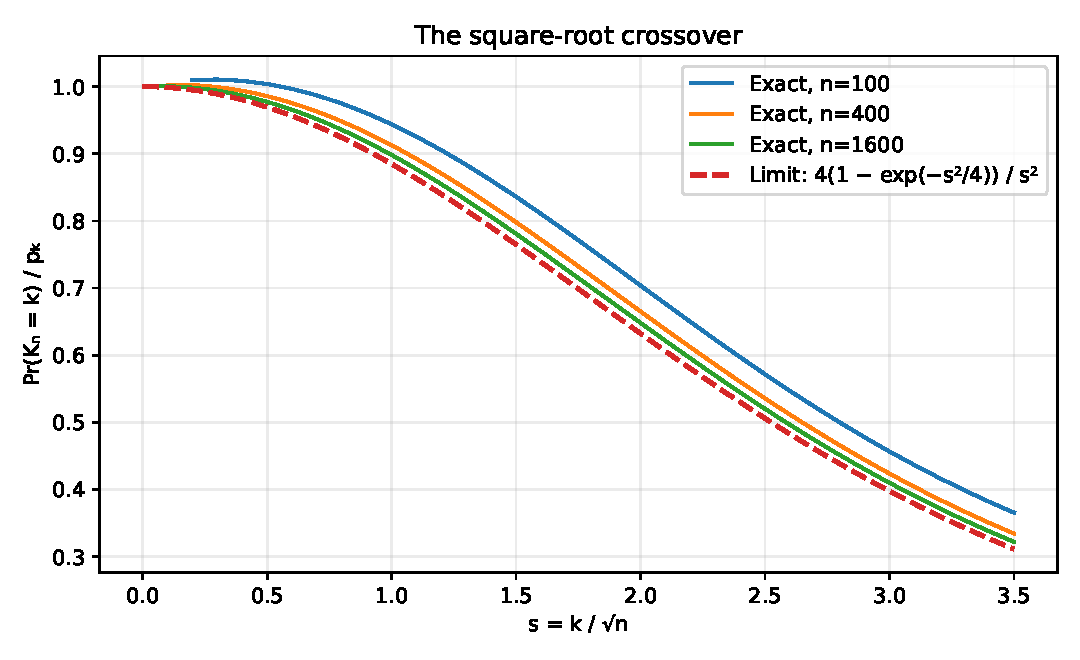
\includegraphics[width=0.88\textwidth]{figures/crossover.pdf}
\caption{Exact normalized column probabilities approach the crossover
function in \eqref{eq:crossover-ratio}. The horizontal coordinate is
$k/\sqrt n$. These curves show why a fixed-$k$ expansion must not be used
uniformly across the whole triangle.}
\label{fig:crossover}
\end{figure}

\section{Two exponential sectors and the near-diagonal regime}

\subsection{Linear rays}
Suppose $\beta=(n-k)/n$ remains in a compact subset of $(0,1)$. Define
\begin{align}\label{eq:ray-exponents}
 h_0(\beta)&=(1+\beta)\log2,\notag\\
 h_1(\beta)&=(1+\beta)\log(1+\beta)-\beta\log\beta,\notag\\
 J(\beta)&=h_0(\beta)-h_1(\beta)>0.
\end{align}
The exact decomposition \eqref{eq:AB-split} gives two separately expandable
exponential sectors. If $\Cat(t)=e^{L_C(t)}$ denotes the formal Catalan
correction series, then
\begin{align}\label{eq:ray-A}
 A_{n,k}&\sim\frac{e^{nh_0(\beta)}}{2\sqrt{\pi\beta n}}
                         \Cat\left(\frac1{\beta n}\right),\\
 B_{n,k}&\sim\sqrt{\frac{\beta}{2\pi(1+\beta)n}}e^{nh_1(\beta)}
                         e^{L_\beta(1/n)},\label{eq:ray-B}
\end{align}
where
\begin{equation}\label{eq:ray-log}
 L_\beta(t)=\sum_{r\ge1}
 \frac{B_{2r}\{(1+\beta)^{1-2r}-\beta^{1-2r}-1\}}
      {2r(2r-1)}t^{2r-1}.
\end{equation}
These follow directly from Stirling's formula, using
$B_{n,k}=\frac\beta{1+\beta}\binom{(1+\beta)n}{\beta n}$.
At every finite order the relative remainders are uniform on the stated
compact sets.

In particular,
\begin{equation}\label{eq:R-ray}
 R_{n,k}\sim \frac{\sqrt2\,\beta}{\sqrt{1+\beta}}e^{-nJ(\beta)}.
\end{equation}
To see $J>0$, note that $J(1)=0$ and
$J'(\beta)=\log(2\beta/(1+\beta))<0$ for $0<\beta<1$.
Near the endpoint,
\begin{equation}\label{eq:J-match}
 J(\beta)=\frac{(1-\beta)^2}{4}+O((1-\beta)^3),
\end{equation}
which explains the square-root crossover from the exponential-sector side.

\begin{remark}[What an exponentially small term does and does not mean]
Equations \eqref{eq:ray-A}--\eqref{eq:ray-B}, together with the exact
identity $T=A-B$, provide a two-sector asymptotic description. A finite
inverse-power approximation to $A$ has an error much larger than $B$.
Thus it would be incorrect to append the leading $B$ term to an arbitrarily
truncated $A$ series and claim the remainder is smaller than $B$. To
resolve the second sector numerically, retain $A$ exactly through its
binomial or gamma expression, or control its approximation to exponentially
small accuracy. Here both sectors are defined exactly before either is
expanded; no resurgence or optimal-truncation theorem is being assumed.
\end{remark}

\subsection{Fixed distance from the diagonal}
For an integer $\ell\ge1$ fixed and $n>\ell$, the exact formula specializes
to
\begin{equation}\label{eq:fixed-deficit}
 \boxed{\displaystyle
 T(n,n-\ell)=2^{n-\ell-1}\binom{2\ell}{\ell-1}
                    -\binom{n+\ell-1}{\ell-1}.}
\end{equation}
The second term is a polynomial in $n$ of degree $\ell-1$. This is a literal
exponential-minus-polynomial expression, not just an asymptotic equivalent.
For example,
\[
 T(n,n-1)=2^{n-2}-1,\qquad
 T(n,n-2)=2^{n-1}-(n+1).
\]
The diagonal itself is $2^{n-1}$. The formulas are valid with their stated
ranges; coincidences with the first zero column at small $n$ are handled
without extra exceptions.

\section{Critical weighting: exact normalization and a beta law}

\subsection{An exact critical partition function}
For $y>0$ define a tilted measure by
\begin{equation}\label{eq:tilt}
 \Prob_{n,y}(K_n=k)=\frac{T(n,k)y^k}{Z_n(y)}.
\end{equation}
The measure at $y=1$ is uniform on $\Av_n(123)$. The value $y=2$ exactly
balances the factor $2^{-k}$ visible in the asymptotics, so it requires a
separate analysis.

\begin{theorem}[Critical normalization and mean]\label{thm:critical-exact}
For $n\ge1$,
\begin{align}\label{eq:Z2}
 Z_n(2)&=(n+2)\binom{2n}{n}-4^n,\\
 \E_{n,2}\frac{K_n}{n}
 &=\frac23+\frac{4^n}{6Z_n(2)}.\label{eq:critical-mean}
\end{align}
In particular,
\begin{align}\label{eq:Z2-expansion}
 Z_n(2)=\frac{4^n\sqrt n}{\sqrt\pi}
 \left(1-\frac{\sqrt\pi}{\sqrt n}+\frac{15}{8n}
       -\frac{31}{128n^2}+\frac{21}{1024n^3}+O(n^{-4})\right),\\
 \E_{n,2}(K_n/n)=\frac23+\frac{\sqrt\pi}{6\sqrt n}+O(n^{-1}).
 \label{eq:mean-expansion}
\end{align}
The partition function has a full expansion obtained by continuing the
central-binomial Stirling series in \eqref{eq:Z2}.
\end{theorem}
\begin{proof}
In terms of $z=\sqrt{1-4x}$, \eqref{eq:F-z} at $y=2$ reduces to
\begin{equation}\label{eq:F2}
 F(x,2)=-1+\frac{3}{2z}-\frac1{z^2}+\frac1{2z^3}.
\end{equation}
Use
\[
 [x^n]z^{-1}=\binom{2n}{n},\qquad
 [x^n]z^{-2}=4^n,\qquad
 [x^n]z^{-3}=(2n+1)\binom{2n}{n}
\]
for $n\ge1$ to obtain \eqref{eq:Z2}.
Differentiating the exact bivariate function gives
\begin{equation}\label{eq:F2-firstmoment}
 \left.y\frac{\partial F}{\partial y}\right|_{y=2}
 =-\frac1{2z}+\frac1{2z^2}-\frac1{2z^4}+\frac1{2z^5}.
\end{equation}
Since
$[x^n]z^{-4}=(n+1)4^n$ and
$[x^n]z^{-5}=\frac{(2n+1)(2n+3)}3\binom{2n}{n}$,
coefficient extraction gives
\[
 \sum_{k=1}^n k2^kT(n,k)
 =\frac{2n(n+2)}3\binom{2n}{n}-\frac n2\,4^n.
\]
Divide by $nZ_n(2)$ and rearrange to prove \eqref{eq:critical-mean}.
Finally, substitute
\[
 \binom{2n}{n}=\frac{4^n}{\sqrt{\pi n}}
 \left(1-\frac1{8n}+\frac1{128n^2}+\frac5{1024n^3}
                     +O(n^{-4})\right)
\]
in the exact expressions. The term $-4^n$ is responsible for the
half-power correction in \eqref{eq:Z2-expansion}.
\end{proof}

\subsection{An elementary positive-measure comparison}
To study the entire distribution, use the same binomial expressions in
\eqref{eq:AB-split} also for $k=1<n$, where $A_{n,1}=B_{n,1}$.
Extend the positive first term to the diagonal by
$A_{n,n}=2^{n-1}$, and put $B_{n,n}=0$. Set
\begin{equation}\label{eq:b-critical}
 b_0=1,\qquad b_\ell=4^{-\ell}\binom{2\ell}{\ell-1}\quad(\ell\ge1).
\end{equation}
Writing $\ell=n-k$ gives
\begin{equation}\label{eq:critical-positive}
 2^kA_{n,k}=\frac{4^n}{2}b_\ell,\qquad 0\le\ell\le n-1.
\end{equation}
These positive weights are close, after normalization, to the actual
critical weights $2^kT(n,k)$.

\begin{lemma}\label{lem:b-partial}
For $N\ge0$,
\begin{equation}\label{eq:b-partial}
 \sum_{\ell=0}^N b_\ell
 =-1+\frac{(2N+1)(N+2)}{N+1}\,
                    \frac{\binom{2N}{N}}{4^N}
 =\frac{2\sqrt N}{\sqrt\pi}-1+O((N+1)^{-1/2}),
\end{equation}
where the last estimate is interpreted with a bounded error also at $N=0$.
Moreover,
\begin{align}\label{eq:AB-totals}
 \sum_{k=1}^n 2^kA_{n,k}
   &=(n+1)\binom{2n}{n}-\frac{4^n}{2},\notag\\
 \sum_{k=1}^n 2^kB_{n,k}
   &=\frac{4^n}{2}-\binom{2n}{n}.
\end{align}
\end{lemma}
\begin{proof}
The finite-sum identity in \eqref{eq:b-partial} is verified at $N=0$ and
then by subtracting its values at $N$ and $N-1$, using the ratio of
successive central binomial coefficients. Stirling's formula gives the
estimate. Multiply the identity with $N=n-1$ by $4^n/2$ and simplify to get
the first equation in \eqref{eq:AB-totals}. Subtract \eqref{eq:Z2} to get
the second.
\end{proof}

\begin{theorem}[Critical beta limit and error]\label{thm:beta}
Under $\Prob_{n,2}$,
\begin{equation}\label{eq:beta-law}
 \frac{K_n}{n}\Rightarrow X,\qquad
 X\sim\Beta(1,\tfrac12),\qquad
 f_X(t)=\frac1{2\sqrt{1-t}}\quad(0<t<1).
\end{equation}
Writing $F_X(t)=1-\sqrt{1-t}$ on $[0,1]$, the distribution functions obey
\begin{equation}\label{eq:beta-error}
 \sup_{0\le t\le1}
 \left|\Prob_{n,2}(K_n/n\le t)-F_X(t)\right|=O(n^{-1/2}).
\end{equation}
All moments converge; in particular the limiting mean is $2/3$ and the
limiting variance is $4/45$.
\end{theorem}
\begin{proof}
Let $\widetilde\Prob_n$ be the measure on $k=1,\ldots,n$ proportional to
$2^kA_{n,k}$. If $A=\sum2^kA_{n,k}$ and $B=\sum2^kB_{n,k}$, then
$Z_n(2)=A-B$. Since all subtracted weights are nonnegative,
\[
 \sum_k\left|\frac{2^kT(n,k)}{A-B}-\frac{2^kA_{n,k}}A\right|
 \le\frac{2B}{A}=O(n^{-1/2}),
\]
by \eqref{eq:AB-totals}. Thus the two measures differ in total variation by
$O(n^{-1/2})$.

Under $\widetilde\Prob_n$, the deficit $\ell=n-k$ has weights $b_\ell$.
The exact partial sum \eqref{eq:b-partial} and its error imply, uniformly
for $0\le u\le1$,
\[
 \widetilde\Prob_n\{(n-K_n)/n\le u\}=\sqrt u+O(n^{-1/2}).
\]
Indeed the numerator is a partial sum through an index within one of $un$,
the denominator is the sum through $n-1$, and the estimates in
\eqref{eq:b-partial} give the claimed uniform error, including both
endpoints. Taking complements and adjusting a possible lattice atom
(which is also $O(n^{-1/2})$) gives the beta law and
\eqref{eq:beta-error}. Since $K_n/n\in[0,1]$, weak convergence implies
convergence of all moments. The beta density directly gives the stated
mean and variance.
\end{proof}

\begin{proposition}[The first bulk correction]\label{prop:beta-correction}
Uniformly for $t$ in any compact subinterval of $(0,1)$,
\begin{equation}\label{eq:beta-first-correction}
 \Prob_{n,2}(K_n/n\le t)
 =F_X(t)+\frac{\sqrt\pi}{\sqrt n}
                      \left(F_X(t)-\frac12\right)+O(n^{-1}).
\end{equation}
This expansion is not asserted uniformly through the endpoints.
\end{proposition}
\begin{proof}
Put $m=\lfloor nt\rfloor$. The positive cumulative weight is
$\frac{4^n}{2}\sum_{\ell=n-m}^{n-1}b_\ell$.
The constant $-1$ cancels in the difference of the two partial sums in
\eqref{eq:b-partial}. Since both endpoints are proportional to $n$,
\[
 \sum_{k\le m}2^kA_{n,k}
 =\frac{4^n\sqrt n}{\sqrt\pi}F_X(t)+O(4^nn^{-1/2}).
\]
For $k>m$, the ratio bound \eqref{eq:R-bound} makes the total $B$ weight
exponentially small compared with $4^n\sqrt n$. Hence
\[
 \sum_{k\le m}2^kB_{n,k}
 =\frac{4^n}{2}-\binom{2n}{n}+O(4^n e^{-c n})
\]
for some $c>0$ depending on the compact interval (a polynomial factor can
be absorbed by reducing $c$). The numerator is therefore
$\frac{4^n\sqrt n}{\sqrt\pi}F_X(t)-4^n/2+O(4^nn^{-1/2})$.
Divide by \eqref{eq:Z2-expansion} to obtain the result. The floor in $m$
changes the leading cumulative expression by only $O(n^{-1})$ after
normalization on the stated compact sets.
\end{proof}

\begin{figure}[tbp]
\centering
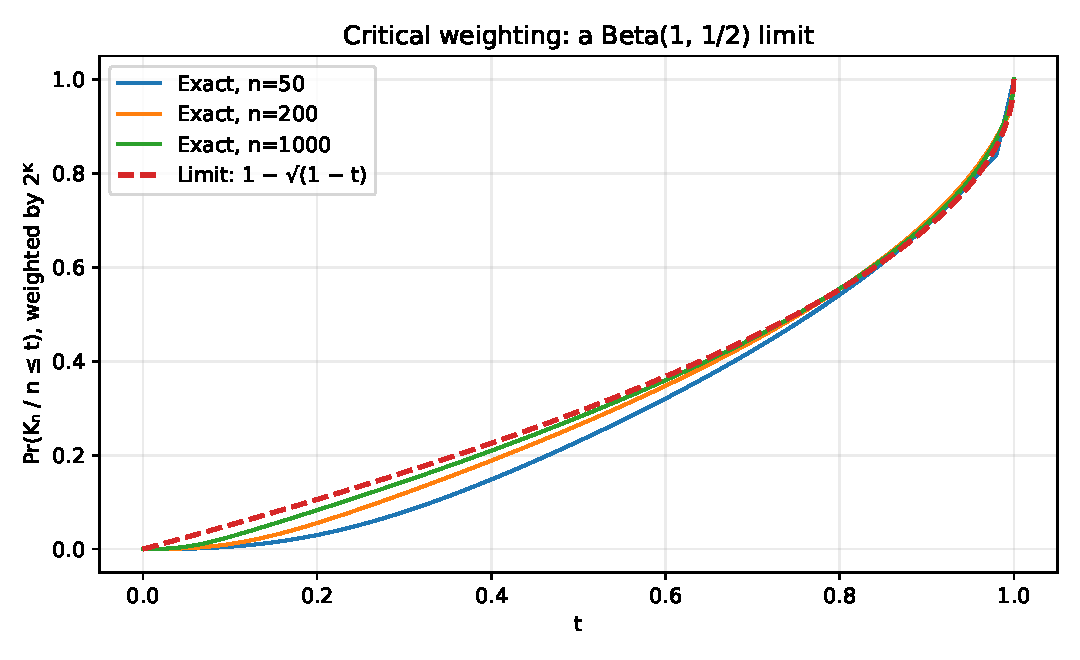
\includegraphics[width=0.88\textwidth]{figures/critical_cdf.pdf}
\caption{At the critical weight $2^{K_n}$, the cumulative distribution of
$K_n/n$ approaches $1-\sqrt{1-t}$. Convergence is only of order
$n^{-1/2}$; the exact mean in \eqref{eq:critical-mean} quantifies one part
of this finite-size effect.}
\label{fig:critical}
\end{figure}

\section{The full tilted phase diagram and its critical window}

\subsection{Below the transition}
\begin{theorem}[Subcritical law]\label{thm:subcritical}
For every fixed $0<y<2$,
\begin{equation}\label{eq:subcritical}
 Z_n(y)=P(y)C_n(1+O_y(n^{-1})),\qquad
 \Prob_{n,y}(K_n=k)\longrightarrow \frac{p_ky^k}{P(y)}.
\end{equation}
The limiting law has an exponential moment, and $K_n/n\to0$ in probability.
The partition function has an all-orders inverse-power expansion at each
fixed subcritical $y$.
\end{theorem}
\begin{proof}
The uniform generating-function estimate \eqref{eq:uniform-pgf} gives the
normalization. Combining it with the fixed-column probabilities gives the
pointwise limit, whose sum is one by definition of $P$. Choose a circle
$|u|=R<2$ with $R>y$. The same coefficient estimates give exponentially
weighted convergence after multiplying by $y^k$, so the family is tight
and has uniformly bounded moments. Expanding \eqref{eq:F-z} to further
odd powers of $z$ gives every fixed inverse-power order of the partition
function by the same transfer argument.
\end{proof}

\subsection{Above the transition}
For $y>2$ put
\begin{equation}\label{eq:super-amplitude}
 q=\sqrt{1-2/y},\qquad
 \mathcal A(y)=\frac12\left(1+\frac1q-C\!\left(\frac1{2y}\right)\right)
              =\frac{q^2+1}{2q(q+1)}.
\end{equation}

\begin{theorem}[Supercritical law]\label{thm:supercritical}
For every fixed $y>2$, there is $0<\eta_y<1$ such that
\begin{equation}\label{eq:super-Z}
 Z_n(y)=\mathcal A(y)(2y)^n(1+O_y(\eta_y^n)).
\end{equation}
The deficit $D_n=n-K_n$ converges in distribution to a nonnegative
integer-valued random variable $D_y$ with
\begin{align}\label{eq:super-law}
 \Prob(D_y=0)&=\frac1{2\mathcal A(y)},\notag\\
 \Prob(D_y=\ell)&=\frac{\binom{2\ell}{\ell-1}}
                         {2\mathcal A(y)(2y)^\ell},\qquad \ell\ge1.
\end{align}
Its generating function is
\begin{equation}\label{eq:super-pgf}
 \E u^{D_y}=\frac{H(u/(2y))}{H(1/(2y))},\qquad
 H(t)=1+(1-4t)^{-1/2}-C(t).
\end{equation}
In particular, $K_n/n\to1$ in probability.
\end{theorem}
\begin{proof}
The pole $\rho=1/(2y)$ of $1/(1-2xy)$ lies strictly inside the Catalan
radius $1/4$. The other denominator in \eqref{eq:main-gf} is nonzero at
$\rho$, since $\rho yC(\rho)=C(\rho)/2<1$. In fact it has no zero in a
slightly larger disk: the bound
$|xyC(x)|\le |x|yC(|x|)$ and continuity suffice.
The numerator of the simple pole is
\[
 \lim_{x\to\rho}(1-2yx)F(x,y)
 =\frac12+\frac{C(\rho)^3}{8y\{1-C(\rho)/2\}}
 =\mathcal A(y).
\]
Subtract $\mathcal A(y)/(1-2yx)$ from $F$. The remainder is analytic in a
disk of radius strictly larger than $\rho$, so Cauchy's coefficient bound
proves \eqref{eq:super-Z}.

For fixed $\ell\ge1$, multiply \eqref{eq:fixed-deficit} by $y^{n-\ell}$
and divide by \eqref{eq:super-Z}. The polynomial term tends to zero
relative to the exponential term, and the limit is
\eqref{eq:super-law}. The diagonal gives the mass at zero. Finally,
\[
 \sum_{\ell\ge1}\binom{2\ell}{\ell-1}t^\ell
 =(1-4t)^{-1/2}-C(t),
\]
so the limiting masses sum to
$H(1/(2y))/(2\mathcal A(y))=1$.
This proves tightness, the asserted law, and its generating function.
\end{proof}
The limiting deficit has an exponential tail since $1/(2y)<1/4$.
At fixed $y>2$, moments converge as well: for $u>1$ sufficiently close to
one, $y/u>2$ and
\[
 \E_{n,y}u^{D_n}=u^n\frac{Z_n(y/u)}{Z_n(y)}
 \longrightarrow\frac{\mathcal A(y/u)}{\mathcal A(y)}
 =\frac{H(u/(2y))}{H(1/(2y))}
\]
uniformly in a neighborhood of $u=1$.

\subsection{Free energy and a finite-size window}
\begin{corollary}\label{cor:freeenergy}
The limiting exponential rate is
\begin{equation}\label{eq:freeenergy}
 f(y):=\lim_{n\to\infty}\frac1n\log Z_n(y)
 =\begin{cases}
 \log4,&0<y\le2,\\
 \log(2y),&y\ge2.
 \end{cases}
\end{equation}
As a function of $\log y$, its one-sided derivatives at $y=2$ are $0$ and
$1$. At exactly $y=2$, the finite-size mean fraction instead converges to
$2/3$, in accordance with the nondegenerate beta law.
\end{corollary}
This derivative jump is the precise sense in which the model has a
first-order transition. It is a description of the proved weighted
combinatorial model, not a claim about a physical system.

\begin{theorem}[Critical window]\label{thm:window}
Let $\lambda\in\mathbb R$ be fixed and $y_n=2e^{\lambda/n}$. Then
\begin{align}\label{eq:window-normalization}
 \frac{Z_n(y_n)}{Z_n(2)}&=M(\lambda)+O_\lambda(n^{-1/2}),\notag\\
 M(\lambda)&=\int_0^1\frac{e^{\lambda t}}{2\sqrt{1-t}}\,\dd t
             =e^\lambda\int_0^1e^{-\lambda u^2}\,\dd u.
\end{align}
Under $\Prob_{n,y_n}$, $K_n/n$ converges to the density
\begin{equation}\label{eq:window-density}
 f_\lambda(t)=\frac{e^{\lambda t}}
                     {2M(\lambda)\sqrt{1-t}},\qquad 0<t<1.
\end{equation}
Both the normalization error and the distribution-function error are
$O(n^{-1/2})$ uniformly for $\lambda$ in a compact real interval.
\end{theorem}
\begin{proof}
The normalization ratio is exactly
$\E_{n,2}\exp(\lambda K_n/n)$. Apply
Theorem~\ref{thm:beta}; integration by parts bounds the difference of
expectations by the distribution-function error times the total variation
of $e^{\lambda t}$ on $[0,1]$. This variation is uniformly bounded for
$\lambda$ in a compact interval. The substitution $t=1-u^2$ gives the
second integral. For the tilted distribution functions, apply the same
argument to $e^{\lambda t}\ind_{t\le a}$ and divide by the normalization,
which remains uniformly bounded away from zero. This proves the stated
limit and rate.
\end{proof}
When $\lambda>0$ one may write
$M(\lambda)=e^\lambda\sqrt\pi\,\operatorname{erf}(\sqrt\lambda)/(2\sqrt\lambda)$;
the integral form is real and nonsingular for every real $\lambda$, with
$M(0)=1$.

\begin{figure}[tbp]
\centering
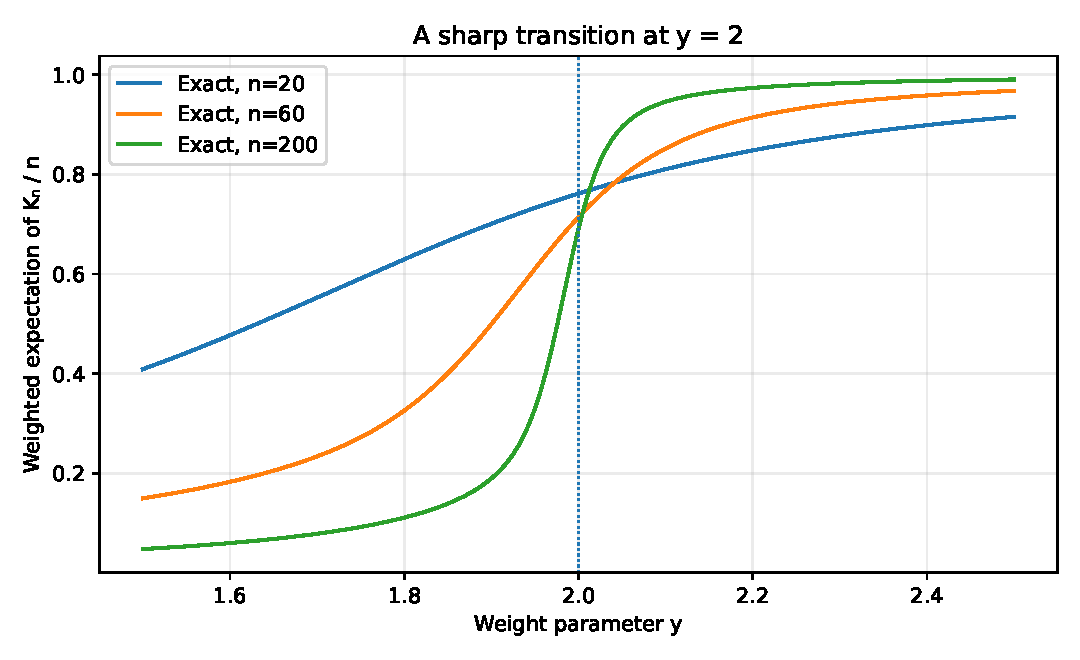
\includegraphics[width=0.88\textwidth]{figures/phase_transition.pdf}
\caption{Exact tilted means for increasing $n$. The limiting mean fraction
is $0$ for fixed $y<2$ and $1$ for fixed $y>2$, with the distinct critical
value $2/3$. The window $y=2e^{\lambda/n}$ resolves the transition rather
than replacing it by a discontinuous finite-$n$ approximation.}
\label{fig:phase}
\end{figure}

\section{Asymptotic inversion and integer thresholds}

\subsection{A natural smooth continuation}
A discrete sequence does not have a unique real inverse without choosing
an interpolation. For fixed $k\ge2$ we use the gamma continuation of the
exact binomial formula:
\begin{align}\label{eq:gamma-continuation}
 T_k(x)
 &=\frac{2^{k-1}\Gamma(2x-2k+1)}{\Gamma(x-k)\Gamma(x-k+2)}\notag\\
 &\quad-\frac{\Gamma(2x-k)}{\Gamma(x-k)\Gamma(x+1)},\qquad x>k.
\end{align}
It equals $T(n,k)$ at all integers $n>k$. The product formula
\eqref{eq:R-product}, now with $\ell=x-k>0$, proves positivity because
each factor is less than one. Differentiated Stirling expansions show that
\begin{equation}\label{eq:log-T}
 \log T_k(x)\sim ax-b\log x+\log A_k^*+
              \sum_{j\ge1}\ell_j(k)x^{-j},
\end{equation}
as an all-orders asymptotic expansion, where
\[
 a=\log4,\qquad b=\frac32,\qquad A_k^*=\frac{p_k}{\sqrt\pi},
 \qquad \ell_1=c_1,\quad \ell_2=c_2-\frac12c_1^2.
\]
Its derivative is $a-b/x+O(x^{-2})>0$ for all sufficiently large $x$.
Thus sufficiently large targets have a unique inverse on the eventual
increasing branch.

\subsection{\texorpdfstring{Lambert-$W$}{Lambert-W} reduction and corrections}
For a target $v\to\infty$, put
\begin{equation}\label{eq:inverse-Y}
 Y=\log(v/A_k^*),\qquad
 N=-\frac ba\,W_{-1}\left(-\frac ab e^{-Y/b}\right).
\end{equation}
The real branch $W_{-1}$, not the principal branch, is required to make
$N\to\infty$. The defining identity for $W$ implies
$ aN-b\log N=Y$; standard branch conventions are recorded in
DLMF \S4.13 \cite{dlmfW}.

\begin{theorem}[Inverse expansion]\label{thm:inverse}
Let $x(v)$ be the eventual increasing inverse of $T_k$. Then
\begin{equation}\label{eq:inverse-two}
 \boxed{\displaystyle
 x(v)=N-\frac{\ell_1}{aN}
       -\frac{\ell_2/a+b\ell_1/a^2}{N^2}+O_k(N^{-3}).}
\end{equation}
An expansion to every order is determined recursively by substituting
$\delta=\sum_{j\ge1}d_jN^{-j}$ in
\begin{equation}\label{eq:inverse-rec}
 a\delta-b\log(1+\delta/N)
       +\sum_{j\ge1}\ell_j(N+\delta)^{-j}=0
\end{equation}
and setting each coefficient equal to zero. At order $N^{-j}$, the new
unknown $d_j$ has coefficient $a\ne0$.
\end{theorem}
\begin{proof}
Write $x=N+\delta$ in \eqref{eq:log-T} and use the exact equation for $N$.
The remaining equation is \eqref{eq:inverse-rec}. At its first two orders,
\[
 ad_1+\ell_1=0,\qquad ad_2-bd_1+\ell_2=0,
\]
which gives \eqref{eq:inverse-two}. Inductively, after the first $J$
coefficients are chosen, the residual in the logarithmic equation is
$O(N^{-J-1})$. Its derivative in $\delta$ is $a+O(N^{-1})$, bounded away
from zero. The mean value theorem transfers the residual to an inverse
error of the same order. Differentiated Stirling remainder bounds justify
the derivatives used here \cite{dlmfgamma}.
\end{proof}
The Lambert quantity itself begins
\begin{equation}\label{eq:inverse-log}
 N=\frac{Y+b\log Y-b\log a}{a}
                +O\left(\frac{\log Y}{Y}\right).
\end{equation}
Repeated substitution, or the standard expansion of $W_{-1}$, expands it
in powers of $Y^{-1}$ with polynomial coefficients in $\log Y$.
Keeping $N$ in Lambert form often gives the more accurate practical
approximation at a fixed number of displayed terms.

\subsection{The rounding issue}
Define the eventual integer threshold
\[
 Q_k(v)=\min\{n\ge k+1:T(n,k)\ge v\}.
\]
For sufficiently large $v$, all earlier finitely many values are below the
target and the continuation is increasing, so $Q_k(v)=\lceil x(v)\rceil$.
However, taking the ceiling of a \emph{truncated} inverse expansion is not
uniformly safe: the exact inverse may lie arbitrarily close to an integer.
If a rigorous remainder bound is $|x(v)-x_J(v)|\le\varepsilon_J$, the
valid conclusion is the bracket
\begin{equation}\label{eq:inverse-bracket}
 \left\lceil x_J(v)-\varepsilon_J\right\rceil
 \le Q_k(v)\le
 \left\lceil x_J(v)+\varepsilon_J\right\rceil.
\end{equation}
An exact binomial evaluation resolves any remaining one- or two-integer
ambiguity. This report proves asymptotic remainder orders; it does not
claim that the floating-point demonstrations alone provide explicit
certified remainder constants or effective monotonicity cutoffs.

\subsection{Inverting the limiting tail}
The limiting discrete law also has a useful inverse asymptotic. Extend its
exact tail formula to large real $m$ and solve
\[
 \varepsilon=2^{-m-2}(m^2+5m+2),\qquad\varepsilon\downarrow0.
\]
Put $u=m+5/2$ and $a_2=\log2$. Then
\begin{equation}\label{eq:tail-equation}
 \varepsilon=\sqrt2\left(u^2-\frac{17}4\right)e^{-a_2u}.
\end{equation}
The leading solution is
\begin{equation}\label{eq:tail-U}
 U=-\frac2{a_2}W_{-1}\left(-\frac{a_2}{2}
                            \sqrt{\frac{\varepsilon}{\sqrt2}}\right).
\end{equation}
Expanding the logarithm of \eqref{eq:tail-equation} about $u=U$ gives
\begin{equation}\label{eq:tail-inverse}
 m=U-\frac52-\frac{17}{4a_2U^2}+O(U^{-3}).
\end{equation}
Indeed, the neglected factor contributes
$\log(1-17/(4U^2))=-17/(4U^2)+O(U^{-4})$ and the derivative of
$2\log u-a_2u$ is $-a_2+2/u$. This determines both the sign and the
coefficient of the correction. Further terms follow recursively. Integer
quantiles require the same rounding care as in
\eqref{eq:inverse-bracket}. This tail inversion concerns the limiting law;
for finite $n$, the exact cumulative formula \eqref{eq:exact-tail} is
available and should be preferred when feasible.

\section{Independent checks, numerical behavior, and reproducibility}

\subsection{Three logically separate checks}
The archive contains \texttt{code/verify.py}, using integer arithmetic for
enumeration and \texttt{sympy}/\texttt{mpmath} for symbolic and numerical
checks. The executed default run performed the following tests.
\begin{enumerate}[leftmargin=2em]
\item \textbf{Direct permutation enumeration.} Every permutation of sizes
$1$ through $9$ was examined: $409{,}113$ permutations in total. A
three-term increasing-subsequence test decides $123$ avoidance. A separate
triple scan finds the largest minimum value of a $132$ occurrence, hence
$K=n-\max\{\hbox{minimum of a $132$ occurrence}\}$, with an empty maximum
of zero. The resulting rows agree with the binomial formula.
\item \textbf{Insertion-state dynamic programming.} An implementation of
the suffix production rule, carrying a flag for whether the first failure
has occurred, checks every row through $n=120$: $7{,}260$ triangle cells.
It verifies Catalan row sums, all cumulative counts, the exact critical
partition function, its first two raw moments, the polynomial factorization,
and the first-order column recurrence. This does not enumerate from the
closed formula being checked.
\item \textbf{Symbolic and high-precision checks.} Symbolic reduction
verifies equality with the posted generating function, the critical
specialization, the limit generating function, and the first three
fixed-column corrections. Numerical tables use $100$ decimal digits and
stable logarithmic evaluation where cancellation is relevant.
\end{enumerate}
All checks passed in the supplied run. These computations are independent
support for the proofs, not a substitute for them and not a proof-assistant
kernel certificate.

\subsection{Illustrative numerical results}
Table~\ref{tab:fixed} reports relative errors
$\hbox{approximation}/T(n,k)-1$. The three approximations retain zero, one,
or two inverse-power corrections in \eqref{eq:all-orders}.
\begin{table}[htbp]
\centering
\small
\begin{tabular}{rrrrr}
\toprule
$k$ & $n$ & Leading term & Through $n^{-1}$ & Through $n^{-2}$\\
\midrule
2 & 100 & $1.3274\cdot10^{-3}$ & $7.5743\cdot10^{-5}$ & $1.4262\cdot10^{-6}$\\
3 & 100 & $6.5417\cdot10^{-4}$ & $1.1810\cdot10^{-4}$ & $3.6291\cdot10^{-6}$\\
5 & 100 & $7.3479\cdot10^{-3}$ & $2.1253\cdot10^{-4}$ & $6.6022\cdot10^{-6}$\\
8 & 100 & $3.7432\cdot10^{-2}$ & $-1.7498\cdot10^{-4}$ & $-2.5042\cdot10^{-5}$\\
\addlinespace
2 & 500 & $2.5304\cdot10^{-4}$ & $2.9808\cdot10^{-6}$ & $1.1250\cdot10^{-8}$\\
3 & 500 & $1.1176\cdot10^{-4}$ & $4.6048\cdot10^{-6}$ & $2.8396\cdot10^{-8}$\\
5 & 500 & $1.4269\cdot10^{-3}$ & $8.2393\cdot10^{-6}$ & $5.0570\cdot10^{-8}$\\
8 & 500 & $7.2969\cdot10^{-3}$ & $-6.0141\cdot10^{-6}$ & $-1.9069\cdot10^{-7}$\\
\bottomrule
\end{tabular}
\caption{Fixed-column asymptotic errors from the independently evaluated
exact formula. All digits shown are rounded from the included CSV file.}
\label{tab:fixed}
\end{table}

Table~\ref{tab:critical} illustrates the slower critical convergence. The
finite mean is always larger than $2/3$ by
\eqref{eq:critical-mean}; the limiting cumulative probability at $1/2$ is
$1-1/\sqrt2\approx0.2928932188$.
\begin{table}[htbp]
\centering
\begin{tabular}{rrr}
\toprule
$n$ & $\E_{n,2}(K_n/n)$ & $\Prob_{n,2}(K_n/n\le1/2)$\\
\midrule
20 & 0.7614630041 & 0.1888612232\\
50 & 0.7197682165 & 0.2294764254\\
100 & 0.7017725312 & 0.2503403803\\
200 & 0.6902952663 & 0.2640357949\\
500 & 0.6809569222 & 0.2753274754\\
1000 & 0.6765433918 & 0.2807136187\\
\addlinespace
Limit & $2/3$ & $1-1/\sqrt2$\\
\bottomrule
\end{tabular}
\caption{Exact critical probabilities, evaluated with arbitrary-precision
arithmetic. The substantial finite-size discrepancy is predicted by the
$n^{-1/2}$ correction, rather than evidence against the beta limit.}
\label{tab:critical}
\end{table}

\subsection{Stable evaluation and complexity}
The two-binomial expression gives a direct exact evaluation with two
binomial coefficients and a power of two. With big integers it is safe
from cancellation, although bit complexity grows with the output length.
For floating-point evaluation when $k$ is small relative to $\sqrt n$,
the two leading binomials nearly cancel. The stable form is
\begin{equation}\label{eq:stable-eval}
 \log T=\log A+\log\bigl(-\operatorname{expm1}(\log R)\bigr),
\end{equation}
using \texttt{log1p} for the factors in \eqref{eq:R-product}.
The verifier uses this form for the gamma continuation and inverse tests.

For a whole table, the suffix-state dynamic program has a straightforward
$O(N^3)$ arithmetic-operation implementation through size $N$, using suffix
sums to aggregate state transitions. This is an operation count, not a
bit-complexity bound; the integer sizes increase with $N$. For an individual
fixed column, the first-order recurrence is usually more convenient after
an initial value is known.

\subsection{Rebuilding the archive}
The source is \texttt{article.tex}; the PDF is compiled with standard
LaTeX packages and references embedded in the source. The figure sources
and CSV data are included. From the archive directory:
\begin{verbatim}
python -m pip install -r requirements.txt
python code/verify.py
python code/make_figures.py
pdflatex -interaction=nonstopmode -halt-on-error article.tex
pdflatex -interaction=nonstopmode -halt-on-error article.tex
\end{verbatim}
The verifier writes \texttt{data/verification\_summary.json} and numerical
CSV files. The supplied \texttt{verification\_log.txt} records the executed
run. No network access is needed after dependencies have been installed.
\texttt{OEIS\_update.txt} contains suggested entry amendments; they have
not been submitted.

\section{Formalization boundary and further research}

\subsection{A concrete path into ProveIt}
The project can be formalized in layers, with a small exact core rather
than an immediate attempt to formalize the entire analytic theory.
First define the restriction to the largest $k$ entries and prove its
monotonicity with respect to pattern containment. Next formalize deletion
and insertion of the minimum as inverse operations, and prove the active
suffix lemma. Finite counting then gives the safe-prefix distribution and
the first-failure convolution. These are the genuinely combinatorial
obligations; a formal manipulation of the conjectured generating function
alone would not establish that it counts the specified permutations.

The subsequent exact algebra is well delimited: Catalan powers, the
binomial telescoper, the entry and tail formulas, and the polynomial-factor
recurrence. Each can be checked without trusting floating-point arithmetic.
The critical partition function and its moment identities can then be
proved by formal-power-series coefficient extraction.

Finally, analytic modules can establish the Stirling expansion, the
uniform coefficient-transfer bound, and the probability limits. The
repository's generic asymptotic scales and differential-block framework
provide a natural home for the formal expansions and inverse recursion
\cite{proveit}. Their existence does not discharge the analytic remainder
obligations. The exact binomial split is especially valuable because it
lets a formal statement distinguish the two exponential sectors without
assuming an unproved summability or resurgent interpretation.

\subsection{Proposed research questions}
The following questions go beyond results established in this report.
They are proposed research directions, not assertions that every one is a
previously published open problem.

\paragraph{1. A family of first-failure statistics.}
Replace $132$ by $1(r+1)r\cdots2$ while retaining global $123$ avoidance.
At a $123$-active site the right-hand suffix decreases, so a new occurrence
is created precisely when at least $r$ entries remain to the right. Thus
safe sites become $j=0,\ldots,r-1$, subject to $j\le d$.
Determine the corresponding first-failure generating functions, explicit
entry formulas where possible, and the critical exponents and limiting
laws. The safe-state process is no longer the same binary reset process;
its analysis is the substantive new step.

\paragraph{2. Joint first-failure and suffix statistics.}
Retain the active suffix length at the first failing insertion and at the
final permutation. Derive a multivariate generating function and determine
whether the critical beta law admits a useful joint limit with either
suffix statistic. The convolution \eqref{eq:convolution} retains the
failing state $j$ and is a starting point, but the joint limit is not
proved here.

\paragraph{3. A fully uniform higher-order theory.}
The leading square-root crossover and the bulk critical correction are
proved above. Develop higher-order expansions that remain uniform as
$k/\sqrt n$ tends to zero or infinity, and match them to the fixed-deficit
region. Similarly resolve the endpoint layers of the critical cumulative
law, where \eqref{eq:beta-first-correction} is not uniform. Explicit
remainder constants would make these expansions directly useful for
certified computation.

\paragraph{4. Complex zeros and finite-size scaling.}
Study the zeros of the polynomial $Z_n(y)$ near $y=2$ and globally.
The critical window suggests that the entire function
$M(\lambda)=e^\lambda\int_0^1e^{-\lambda u^2}\,\dd u$ should govern local
complex scaling. Establish the requisite complex-uniform convergence,
locate its zeros, and connect them to the accumulation of zeros of $Z_n$.
Real-window convergence alone does not supply this theorem.

\paragraph{5. The polynomial factors $H_k$.}
Determine the geometry and asymptotic distribution of the zeros of $H_k$
as $k\to\infty$, and seek structural coefficient bases or recurrences
that explain them. Positivity on $n>k$ and the leading coefficient are
proved here; real-rootedness or any broader zero-location claim is not
assumed. A useful outcome could be sharper rational bounds on column
ratios.

\paragraph{6. Effective inverse certificates.}
Make the inverse theorems effective by producing explicit monotonicity
cutoffs and remainder constants, then combine interval evaluation of
$W_{-1}$ and gamma functions with exact binomial checks. The goal is a
certified threshold algorithm, with a proof that a short interval contains
the answer, rather than an unqualified rounding of an asymptotic formula.

\paragraph{7. Direct bijections to familiar Catalan objects.}
Translate the first-failure parameter into a natural Dyck-path or ordered-tree
statistic, preferably preserving the two low-column interpretations.
The insertion tree already supplies an encoding, but a transparent
object-level bijection may explain the two-binomial cancellation and the
critical beta law without generating functions.

\paragraph{8. Kernel-checked enumeration and reusable analytic interfaces.}
Implement the exact layer in Lean and use it as a test case for a reusable
interface between finite combinatorial enumeration, rational generating
functions over the Catalan extension, and asymptotic statements with
explicit remainders. The distinction between exact algebraic identities,
formal transseries, and analytic estimates should remain visible in the
theorem signatures and audit output.

\subsection{Conclusion}
The posted conjecture for A273821 is accessible through the first insertion
that creates a forbidden pattern. That combinatorial event leads to a
positive Catalan convolution, a telescoping binomial formula, and a complete
fixed-column asymptotic expansion. It also reveals behavior invisible in
the original growth-rate comment: a square-root crossover, a precise
separation of exponential sectors, and a weighted transition from bounded
first-failure time to bounded final deficit, with a beta law exactly at
criticality. The exact formulas, rather than numerical extrapolation,
support every asserted asymptotic regime.

\appendix
\section{Additional exact identities and coefficients}

\subsection{The OEIS triangle recurrence}
With the boundary conventions stated in Section~1, the proved generating
function also verifies the recurrence displayed in the OEIS entry:
\begin{align}\label{eq:oeis-rec}
 T(n,k)={}&3T(n-1,k-1)-2T(n-2,k-2)\notag\\
 &+T(n,k+1)-2T(n-1,k)+\ind_{k=2}C_{n-2},
 \qquad n\ge3,\ 2\le k\le n.
\end{align}
Together with $T(1,1)=1$, $T(2,2)=2$, and the zero boundaries, it computes
rows from right to left. It is a consequence of the counting proof, not
an assumption used to derive it. One verification is to insert the
binomial expression and use Pascal's identity; another is to multiply
\eqref{eq:main-gf} by the recurrence kernel and compare coefficients.

\subsection{A third fixed-column correction}
The coefficient generator \eqref{eq:all-engine} gives
\begin{equation}\label{eq:c3}
 c_3(k)=-\frac{
 \begin{gathered}
 2k^7-38k^6+130k^5+270k^4-3657k^3\\[-2pt]
 {}+26093k^2-34725k+13860
 \end{gathered}}
 {3072(k+4)}.
\end{equation}
This coefficient is independently regenerated in the symbolic check, rather
than merely inserted as a numerical fit. For higher orders, the power sums
in \eqref{eq:ab} and the exponential recurrence
\eqref{eq:exp-rec} are preferable to increasingly large printed polynomials.

\subsection{The second critical raw moment}
A second application of $y\partial_y$ gives
\begin{equation}\label{eq:second-gf}
 \left.(y\partial_y)^2F\right|_{y=2}
 =\frac1{2z}-\frac3{2z^2}+\frac2{z^3}-\frac3{2z^4}
            +\frac1{2z^5}-\frac1{z^6}+\frac1{z^7}.
\end{equation}
Consequently,
\begin{align}\label{eq:critical-second}
 \sum_{k=1}^n k^2 2^kT(n,k)
 ={}&\frac{2(4n^3+23n^2+63n+30)}{15}\binom{2n}{n}\notag\\
 &-\frac{(n+2)(n+4)}2\,4^n.
\end{align}
Together with \eqref{eq:Z2} and \eqref{eq:critical-mean}, this provides an
exact finite-$n$ variance and another independent check on the limiting
variance $4/45$ after scaling by $n^2$.

\section{Source and claim ledger}
\begin{longtable}{>{\raggedright\arraybackslash}p{0.23\textwidth}>{\raggedright\arraybackslash}p{0.69\textwidth}}
\toprule
Item & Status and use\\
\midrule
\endhead
A273821 definition and conjecture & Primary OEIS entry retrieved October 1,
2026. The entry labels its generating function conjectural and suggests
fixed-column growth $4$. The present report proves both claims from the
permutation definition.\\[4pt]
A000245 and A071718 & Known companion columns with the initial exceptions
specified in \eqref{eq:companions}. Their existing leading asymptotics are
acknowledged, not claimed as new.\\[4pt]
Catalan insertion machinery & Proved directly in Sections 2--3. General
Catalan and singularity-analysis methods are established background.\\[4pt]
Stirling and transfer estimates & Standard analytic inputs, cited to DLMF
and \emph{Analytic Combinatorics}; their hypotheses are checked in the uses
above. Coefficients and model-specific deductions are derived here.\\[4pt]
Exact formulas and limit laws & Conventional proofs supplied in this report;
independent computational checks supplied in the archive. No Lean certificate
is claimed.\\[4pt]
ProveIt connection & The inspected transseries project supplies methodological
context and a possible formalization destination, not an assumed proof of
any theorem in this report. Repository tree inspected at commit
\texttt{291fbe6bb4477e0cb2131f1e041b12a9abe363fd}.\\[4pt]
Novelty search & Targeted identifier/statistic searches and repository searches
found no independent proof of the posted conjecture. This is not an exhaustive
bibliographic certification.\\[4pt]
Proposed extensions & Section 13 distinguishes further research from theorems
actually proved. The OEIS amendment file is a draft, not a submitted edit.\\
\bottomrule
\end{longtable}

\clearpage
\begin{thebibliography}{9}
\raggedright
\bibitem{oeis273821}
David Callan, \emph{OEIS A273821: a triangle of $123$-avoiding permutations
refined by $132$ avoidance of their largest entries}, The On-Line
Encyclopedia of Integer Sequences, entry introduced May 31, 2016.
Retrieved October 1, 2026. \url{https://oeis.org/A273821}.

\bibitem{oeis245}
The OEIS Foundation Inc., \emph{OEIS A000245}, including its factorial
formula, generating function, and leading asymptotic. Retrieved October 1,
2026. \url{https://oeis.org/A000245}.

\bibitem{oeis71718}
The OEIS Foundation Inc., \emph{OEIS A071718}, including its Catalan
expression and leading asymptotic. Retrieved October 1, 2026.
\url{https://oeis.org/A071718}.

\bibitem{flajolet}
Philippe Flajolet and Robert Sedgewick,
\emph{Analytic Combinatorics}, Cambridge University Press, 2009,
especially Chapter VI (singularity analysis).
Author-maintained companion site: \url{https://ac.cs.princeton.edu/}.

\bibitem{dlmfgamma}
NIST Digital Library of Mathematical Functions,
\emph{\S5.11: Asymptotic Expansions of the Gamma Function},
including the logarithmic Stirling expansion and remainder estimates.
Retrieved October 1, 2026. \url{https://dlmf.nist.gov/5.11}.

\bibitem{dlmfW}
NIST Digital Library of Mathematical Functions,
\emph{\S4.13: Lambert $W$-Function}, including real branches and asymptotic
expansions. Retrieved October 1, 2026. \url{https://dlmf.nist.gov/4.13}.

\bibitem{proveit}
Vladimir Reshetnikov, \emph{ProveIt}, transseries project README and
repository tree inspected October 1, 2026.
\url{https://github.com/VladimirReshetnikov/ProveIt}.
Project path: \texttt{Analysis/Transseries/README.md}.
The README records the independent transseries library, canonical inversion
volume, and combinatorial companion; these are contextual rather than
logical dependencies of the proofs here.
\end{thebibliography}

\end{document}
